\chapter{\IfLanguageName{dutch}{Stand van zaken}{State of the art}}%
\label{ch:stand-van-zaken}

De orderverwerking binnen 3D-printproductie, is een proces dat helpt aan de efficiëntie en consistentie van productie. Kleinschalige e-\-commerce bedrijven werken vaak handmatig voor het verwerken van orders, zoals het controleren of er een nieuwe bestellingen zijn binnengekomen. Om dat vervolgens te verwerken, zodat de printer kan starten. Vaak worden er ook Excel-bestanden of papieren lijsten gebruikt om orders bij te houden, wat tijdrovend en foutgevoelig kan zijn. Door de voortdurende ontwikkeling van technologie is het automatiseren van deze processen interessant. Zo kan er een proces worden opgezet dat dit met behulp van een Pipeline met API-integraties regelt. Dit vermindert fouten en versnelt het bedrijfsproces. 

\section{Vergelijkbare studies}%
\label{sec:Vergelijkbare studie}

Er zijn al een aantal verschillende vergelijkbare studies die zich richten op de automatisering van productie binnen 3D-printen. In een onderzoek van Maarten van Welsem bespreekt hij wat de impact is van 3D-printtechnologieën op de supply chain. Het beschrijft hoe automatisering een grotere flexibiliteit kan bieden, vooral voor reserveonderdelen en ondemand productie~\autocite{emerce3DprintSupplyChain}. Verder wordt er in een artikel van 3D Print Magazine beschreven hoe de automatisering binnen Europese 3D-printbedrijven hen helpt om mee te kunnen met andere bedrijven, door efficiënt aan de slag te gaan met complexe productieschema's. Ziggzagg hebben een grootschalig bedrijf en werken maar met 12 personen om al die printers te besturen door de automatisatie~\autocite{3dprintmagAutomation}. 

\newpage

\section{3D-printen \& industrie}%
\label{sec:3D-printen & industrie}

\subsection{Inleiding}
3D-printen, ook wel bekend als Additive Manufacturing (AM), is een technologie die in de afgelopen decennia een enorme ontwikkeling heeft doorgemaakt \autocite{3dPrintingIndustry}. Deze techniek maakt het mogelijk om driedimensionale objecten laag voor laag op te bouwen met behulp van verschillende materialen zoals plastiek, metaal en hars. In dit onderzoek bespreken we de Bambu Lab X1C-Carbon als specifieke use case.

\subsection{Wat is 3D-Printen?}
3D-printen is een proces waarbij digitale 3D-modellen worden omgezet in fysieke objecten door opeenvolgende lagen materiaal neer te leggen. Dit proces verschilt van traditionele technieken zoals frezen en lazeren, omdat het materiaal alleen wordt toegevoegd waar nodig \autocite{3dPrintingIndustry}. Er zijn verschillende 3D-printtechnieken zoals:
\\
\begin{wrapfigure}{r}{0.3\textwidth} % Verklein de breedte van de afbeelding
    \centering
    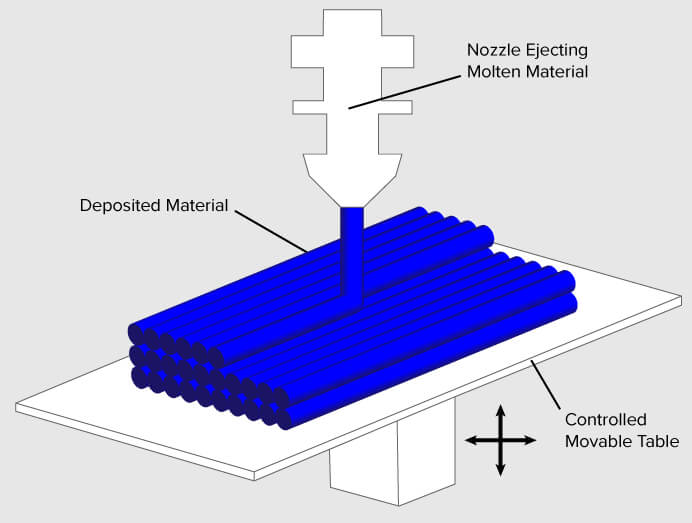
\includegraphics[width=0.8\linewidth]{Foto's/FDM}
    \caption{FDM printtechniek. Bron:~\autocite{3dprintingImage}}
    \label{fig:fdm}
\end{wrapfigure}
\begin{itemize}
    \item Fused Deposition Modeling (FDM)
    \item Stereolithografie (SLA)
    \item Selective Laser Sintering (SLS)
    \item Digital Light Processing (DLP)
\end{itemize}
Voor dit onderzoek wordt de FDM-printtechniek gebruikt, omdat het makkelijk, goedkoop is en nog steeds een kwalitatief resultaat levert voor verkoop aan klanten.

\subsection{Geschiedenis van 3D-Printen}
De oorsprong van 3D-printen gaat terug tot de jaren 80, toen Charles Hull stereolithografie (SLA) ontwikkelde. Gedurende de jaren 90 en 2000 zagen we de opkomst van FDM en andere technologieën die later betaalbaar werden voor consumenten \autocite{3dPrintingIndustry}. Sindsdien is 3D-printen steeds toegankelijker geworden en wordt het gebruikt in industrieën zoals luchtvaart, geneeskunde en de automobielsector.

\newpage
\subsection{De 3D-Printing Industrie}
De 3D-printindustrie groeit snel en kan voor veel toepassingen gebruikt worden. Grote bedrijven zoals HP en Stratasys ontwikkelen industriële printers, terwijl merken zoals Bambu Lab zich richten op hoogwaardige consumenten- en prosumer-markten \autocite{3dPrintingIndustry}. Automatisering speelt een grote rol in de efficiëntie en snelheid van productie.

\subsection{Use Case: Bambu Lab X1C-Carbon}
\begin{wrapfigure}{r}{0.3\textwidth} % Verklein de breedte van de afbeelding
    \centering
    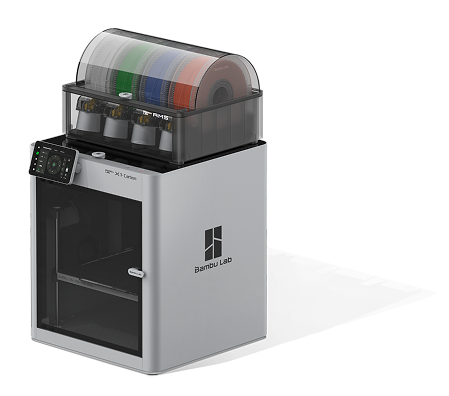
\includegraphics[width=0.8\linewidth]{Foto's/X1C}
    \caption{Bambu Lab X1C-Carbon 3D-printer. Bron::~\autocite{bambulabImage}}
    \label{fig:x1c}
\end{wrapfigure}
De Bambu Lab X1C-Carbon is een geavanceerde 3D-printer die speciaal is ontworpen voor snelheid en precisie. Enkele kenmerken zijn:
\begin{itemize}
    \item Hoge printsnelheid tot 500 mm/s
    \item CoreXY mechanisme voor stabiliteit
    \item Ondersteuning voor meerdere materialen, inclusief met koolstof versterkte filamenten
\end{itemize}
Deze printer werkt samen met de Bambu Studio slicer, een software die 3D-modellen omzet in printbare instructies \autocite{bambulabX1Carbon}.


\newpage

\section{E-commerce}%
\label{sec:E-commerce}

E-commerce is de laatste jaren uitgegroeid tot een van de belangrijkste manieren voor bedrijven om producten en diensten aan te bieden aan klanten. De opkomst van het internet en de ontwikkeling van digitale betalingssystemen hebben het gemakkelijker gemaakt voor bedrijven van elke omvang om een online winkel te starten. E-commerce omvat verschillende modellen, van B2C (Business to Consumer) tot B2B (Business to Business), en biedt tal van voordelen zoals bereikbaarheid, lage operationele kosten en de mogelijkheid om 24/7 actief te zijn~\autocite{bang2024}.

\subsection{Waarom Shopify?}

\begin{wrapfigure}{r}{0.3\textwidth}
    \centering
    
\includegraphics[width=0.8\linewidth]{Foto's/shopify-store}
    \caption{Shopify Logo. Bron:~\autocite{shopifyImage}}
    \label{fig:shopify-store}
\end{wrapfigure}


Shopify is een gebruiksvriendelijk platform dat toegankelijk is voor ondernemers zonder uitgebreide technische kennis. De interface is intuïtief en vereenvoudigt het proces van het opzetten en beheren van een online winkel. Daarnaast biedt Shopify uitgebreide functies, zoals productbeheer, betalingsverwerking, voorraadbeheer en marketingtools, waardoor ondernemers alle nodige middelen hebben om hun webshop efficiënt te runnen.
\\\\
Een ander belangrijk aspect van Shopify is de schaalbaarheid. Het platform is geschikt voor zowel kleine als grote bedrijven en kan eenvoudig meegroeien naarmate het bedrijf zich ontwikkelt. Hierdoor blijft Shopify een duurzame keuze voor ondernemingen die hun online aanwezigheid willen uitbreiden.
\\\\
Bovendien hecht Shopify veel belang aan beveiliging. Het platform voldoet aan de hoogste normen voor gegevensbeveiliging en is PCI-compliant, wat betekent dat klantgegevens en betalingsinformatie op een veilige manier worden verwerkt en beschermd~\autocite{bang2024}.

\newpage

\subsection{De Rol van Shopify in Dit Onderzoek}

In dit onderzoek wordt Shopify gebruikt om een webshop te bouwen waar specifieke producten te koop worden aangeboden. Shopify biedt de benodigde tools voor het eenvoudig beheren van producten, betalingen en klanten.

\subsubsection{De Voordelen voor Dit Project}
\begin{itemize}
     \item \textbf{Eenvoudig externe integratie:} Het is mogelijk om te gaan verbinden met een API, dit maakt het zeer handig om een pipeline aan te binden.
    \item \textbf{Eenvoudig productbeheer:} Eenvoudig om bestanden en andere digitale producten toe te voegen, beheren en verkopen via de webshop.
    \item \textbf{Betalingsverwerking:} Ondersteunt verschillende betalingsmethoden, waardoor klanten eenvoudig kunnen betalen voor hun aankopen.
    \item \textbf{Flexibiliteit en aanpasbaarheid:} De webshop kan worden aangepast aan de specifieke behoeften van het project, van het ontwerp tot de integratie van de gewenste functies~\autocite{bang2024}.
\end{itemize}

\section{API}%
\label{sec:api}

Het gebruik van API’s is ook essentieel, zo gebruiken we de \textbf{Bambu Labs-API}, die biedt een Python API voor interactie met Bambu Lab 3D Printers~\autocite{bambulabsAPI}. Er is ook de Shopify API nodig voor de bestellingen te volgen. Dat is de \textbf{Airbyte Shopify Loader} dit zorgt ervoor dat de inkomende bestellingen geladen kunnen worden~\autocite{ilamaIndexShopify}. 

\subsection{Wat is een API?}

Een API (Application Programming Interface) is een set van regels en protocollen die softwaretoepassingen in staat stelt met elkaar te communiceren. API’s fungeren als tussenpersonen tussen twee systemen, zodat ze gegevens en functionaliteit kunnen uitwisselen. API’s maken het mogelijk om interacties tussen systemen te vereenvoudigen zonder dat de gebruiker direct tussenbeide hoeft te komen.~\autocite{aws2024}.\\

API’s kunnen verschillende taken uitvoeren, van het ophalen van gegevens uit een database tot het uitvoeren van complexe berekeningen. De integratie van API’s in een systeem maakt het mogelijk om verschillende softwarecomponenten te verbinden, wat zorgt voor een robuustere en flexibele toepassing~\autocite{rapidapi2024}.

\newpage

\subsection{De mogelijkheden met de Bambu Labs-API}

\begin{itemize}
    \item Verbind en bedien Bambu Lab 3D-printers programmatisch. 
    \item Houd de printerstatus in realtime in de gaten. 
    \item Voer opdrachten uit en beheer afdruktaken via Python-code. 
    \item Eenvoudige installatie en integratie met Python\--omgevingen. 
\end{itemize}

Het kan bijvoorbeeld met het commando \texttt{bambulabs\_api.Printer.start\_print} de printer s\-tarten als  de juiste variabelen meegegeven worden~\autocite{bambulabsAPI}  

\subsection{De mogelijkheden met de Shopify-API:}

De Shopify-plugin biedt een eenvoudige manier om bestellingen te beheren en te synchroniseren binnen een geautomatiseerde workflow. Dankzij deze integratie kunnen bestellingen die via Shopify binnenkomen eenvoudig worden gevolgd en verwerkt zonder dat directe API-aanroepen nodig zijn.

\begin{itemize} 
    \item Bestellingen automatisch te synchroniseren en te beheren binnen het Shopify-dashboard. 
    \item Ordergegevens op te halen, inclusief productinformatie, klantgegevens en verzendstatus. 
    \item Eenvoudig koppelingen te maken met externe systemen of toepassingen die Shopify ondersteunen. 
\end{itemize}

Deze functionaliteit maakt het mogelijk om de ordergeschiedenis bij te houden en processen te automatiseren zonder diepgaande technische integratie. Voor Python-ontwikkelaars biedt Shopify een officiële Python API, waarmee ontwikkelaars eenvoudig toegang krijgen tot ordergegevens en andere functionaliteiten van Shopify~\cite{shopifyPythonAPI}.

\newpage

\section{Pipelines}%
\label{sec:pipelines}

Een \textbf{pipeline} is een methode om een reeks bewerkingen of processen te organiseren die gegevens verwerken. De uitvoer van de ene bewerking wordt de invoer van de volgende, totdat het uiteindelijke resultaat is verkregen~\autocite{pythonPipelinesThakur}. Pipelines spelen een cruciale rol bij het stroomlijnen van processen, vooral wanneer verschillende systemen of technologieën samenwerken.\\

Volgens~\autocite{thesusVirtanen} bieden pipelines een efficiënte manier om taken te automatiseren en consistente resultaten te garanderen. Vaak worden ze gecombineerd met containerisatieplatforms zoals \textit{Docker} om applicaties en afhankelijkheden te isoleren en consistentie over verschillende omgevingen te waarborgen~\autocite{ijrasetCICDPipeline}. Daarnaast versnellen CI/CD-pipelines niet alleen ontwikkelingsprocessen, maar verbeteren ze ook foutdetectie en kwaliteitsborging. Bekende tools zoals \textbf{Jenkins}, \textbf{GitLab CI/CD} en \textbf{AWS CodePipeline} maken gebruik van geautomatiseerde tests en \textit{zero-downtime deployment} om betrouwbare, veilige en schaalbare processen te garanderen~\autocite{ijrasetFileServe}.\\

In dit onderzoek worden \textbf{GitLab CI/CD}, \textbf{Bitbucket Pipelines}, \textbf{Jenkins}, \textbf{GitHub Actions} en \textbf{Google Cloud Build} geanalyseerd op basis van flexibiliteit, integratiemogelijkheden en gebruiksgemak. Dit helpt bij het bepalen van de meest geschikte pipeline voor de automatiseringsoplossing. Verder onderzoek richt zich op mechanismen om de pipeline continu betrouwbaar te houden, wat essentieel is voor een robuuste CI/CD-oplossing.

\subsection{CI/CD Pipelines}
\textbf{CI/CD (Continuous Integration en Continuous Deployment)} pipelines versnellen softwareontwikkeling en verhogen de betrouwbaarheid door automatische code-tests en deployments zonder handmatige tussenkomst. Degene die worden onderzocht zijn:

\begin{itemize}
    \item \textbf{Jenkins}: Open-source automatiseringsserver met flexibele configuraties en plugins voor CI/CD-processen.
    \item \textbf{GitHub Actions}: Automatiseringsplatform geïntegreerd in GitHub voor het definiëren van workflows.
    \item \textbf{Bitbucket Pipelines}: DevOps-tool voor automatische code-integratie en deployment naar verschillende omgevingen.
    \item \textbf{GitLab CI/CD}: Geïntegreerde oplossing voor builds, tests en deployments via YAML-configuratiebestanden.
    \item \textbf{Google Cloud Build}: Cloudgebaseerde build- en testomgeving voor betrouwbare en schaalbare softwaredistributie.
\end{itemize}

Deze tools maken gebruik van \textit{geautomatiseerde tests} en \textit{zero-downtime deployment} om softwareontwikkeling te optimaliseren. De reden dat deze pipelines worden getest, is omdat ze vaak worden gebruikt in bestaande projecten en bedrijven, en omdat ze goed gedocumenteerd zijn. De keuze is gebaseerd op factoren zoals bekendheid in de industrie, prijs, beschikbare documentatie en eerder onderzoek naar de effectiviteit van verschillende pipelines.
\\\\
Zo bespreekt het onderzoek van~\cite{virtanen2021} hoe verschillende CI/CD-oplossingen scoren op deze criteria. Daarbij is gekeken naar welke pipelines populair zijn binnen bedrijven en open-source projecten, welke kosten eraan verbonden zijn, en hoe toegankelijk en volledig de documentatie is. Dit onderzoek hielp om een gefundeerde keuze te maken voor de meest geschikte pipelines binnen dit project.

\subsubsection{Jenkins}
Jenkins is een open source automatiseringsserver, Jenkins is bachikbaar als een servlet een traditionele servletcontainer, Docker-image en als standalone toepassing via de Java Runtime Environment~\autocite{jenkinsinstalling}. 
\\\\
Jenkins Pipeline is een reeks plug-ins die de implementatie en de integratie van CI/CD-pipelines in Jenkins ondersteund. De pipeline biedt een set hulpmiddelen voor het modelleren van een eenvoudige en complexe "Pipeline-as-code" via de Pipeline DSL-syntaxis, Door de definitie van een Jenkins-pijplijn uit te schrijven in een tekstbestand genaamd 'Jenkinsfile'. "Pipeline-as-code" maakt het mogelijk om de pipeline als onderdeel van het project te verwerken, deze op te slaan in versiebeheer en te beoordelen als elke andere code. De pipeline kan verschillende fasen bevatten, zoals bouwen, testen en implementeren, en kan worden uitgebreid met gedeelde bibliotheken en Docker-ondersteuning.~\autocite{jenkinspipeline}.De Jenkinsfile is een essentieel onderdeel van de Jenkins Pipeline, waarin je het hele proces van continue integratie en levering definieert. Het is een tekstbestand dat de stappen beschrijft die uitgevoerd moeten worden, van het bouwen van de code tot het testen en implementeren ervan. Er zijn twee hoofdtypen syntaxis voor de Jenkinsfile: Declarative en Scripted. Declarative syntax is gebruiksvriendelijker en biedt een duidelijke structuur, terwijl Scripted syntax meer flexibiliteit biedt voor complexe workflows. Het gebruik van een Jenkinsfile stelt teams in staat om hun pijplijnen versiebeheer te geven, wat zorgt voor transparantie en samenwerking bij het ontwikkelen van software.~\autocite{jenkinsjenkinsfile}
\\\\
In Jenkins is het beheren van credentials cruciaal voor het veilig uitvoeren van taken die authenticatie vereisen, zoals toegang tot externe repositories, API’s, of cloudservices. Jenkins biedt een ingebouwd systeem voor het opslaan en beheren van credentials, waarbij gevoelige informatie zoals wachtwoorden en toegangstokens veilig wordt opgeslagen. Jenkins-credentialbeheer wordt standaard geleverd via de Jenkins Credentials Binding-plugin. Inloggegevens die worden opgeslagen met de Credential Binding-plugin kunnen overal binnen de applicatie worden benaderd, of de toegang tot de inloggegevens kan worden beperkt per pipeline-item, Jenkins-gebruiker of -groep.~\autocite{jenkinscredentials}.

\newpage

\subsubsection{GitHub Actions}

GitHub Actions is een platform voor continue integratie en continue levering (CI/CD) dat je in staat stelt om je bouw-, test- en implementatieprocessen te automatiseren. Je kunt workflows maken die elke pull request in je repository bouwen en testen, of samengevoegde pull requests naar productie implementeren. Workflows bestaan uit jobs en hebben stappen en stappen hebben acties. Workflows worden uitgevoerd op runners (Figuur 2.4). Een runner is een applicatie die wordt uitgevoerd op servers. Runners kunnen worden gehost en beheerd door GitHub of op zelf-gehoste machines~\autocite{githubActionsIntro}.
\\\\
Workflows worden opgesteld met een YAML-bestand dat zich bevindt in de map “.github/workflows”. De opbouw van een workflow wordt in grote lijnen weergegeven in (Figuur 2.4). De YAML-structuur is zo ingericht dat deze een job bevat die begint bij een specifieke gebeurtenis, zoals het openen van een pull request op een bepaalde branch of een handmatige trigger van de workflow door de gebruiker. Elke job kan verschillende stappen omvatten, waarbij gebruik gemaakt kan worden van GitHub-acties. Acties zijn vooraf gedefinieerde functionaliteiten die je kunt combineren om de gewenste workflow te creëren. Gebruikers hebben de mogelijkheid om acties te hergebruiken die door de GitHub-community zijn ontwikkeld, of ze kunnen hun eigen acties vanaf het begin opzetten. Dit biedt veel flexibiliteit en mogelijkheden om workflows op maat te maken, afgestemd op de specifieke behoeften van een project of team.~\autocite{githubActionsIntro}.

\begin{figure}[H]
    \centering
    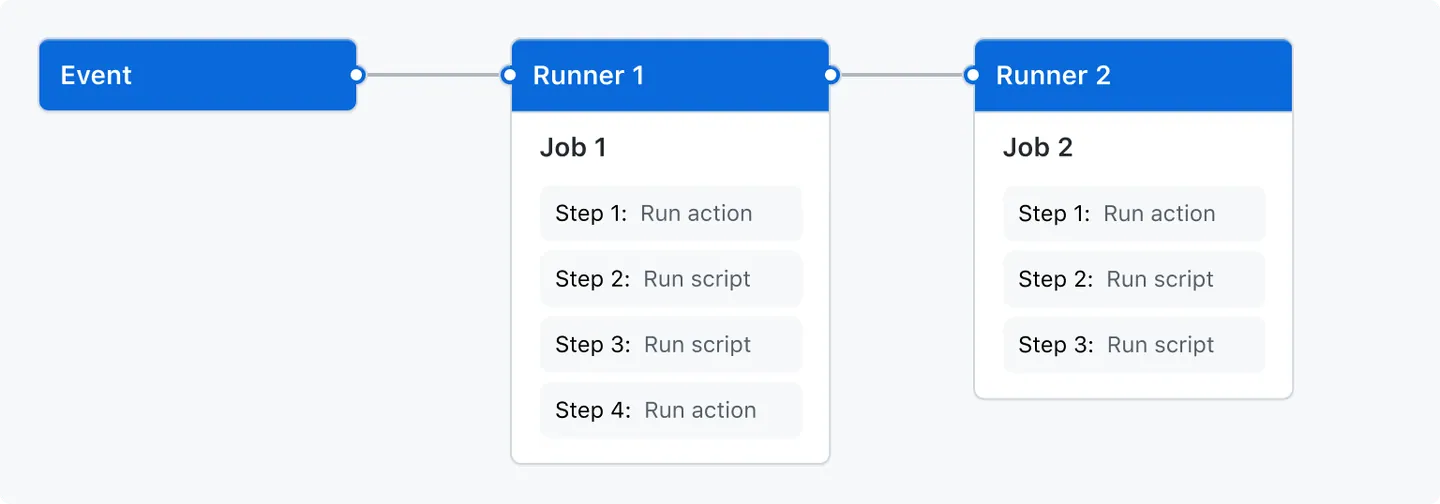
\includegraphics[width=0.8\linewidth]{Foto's/overview-actions-simple.png}
    \caption{GitHub Actions workflow-structuur. Bron: ~\autocite{githubActionsIntro}.}
    \label{fig:workflow-structuur}
\end{figure}

\\\\
GitHub Actions biedt een bepaald aantal opslagruimte en gratis minuten die afhangen van het contractniveau met GitHub. Bijvoorbeeld, GitHub Free bevat slechts 500 megabytes aan opslagruimte en 2.000 minuten runtime voor jobs per maand. De minuten worden ook vermenigvuldigd afhankelijk van het besturingssysteem van de gebruikte runner, zoals te zien in Tabel 1~\autocite{githubActionsBilling}.
\\\\
\begin{table}[h!]
    \centering
    \begin{tabular}{|l|l|}
        \hline
        \textbf{Besturingssysteem} & \textbf{Vermenigvuldiger voor minuten} \\ \hline
        Linux                       & 1                                     \\ \hline
        macOS                       & 10                                    \\ \hline
        Windows                     & 2                                     \\ \hline
    \end{tabular}
    \caption{Vermenigvuldiger van build-minuten voor verschillende besturingssystemen~\autocite{githubActionsBilling}.}
    \label{tab:minutes_multiplier}
\end{table}

\newpage

\subsubsection{Bitbucket Pipelines}

Bitbucket Pipelines is een cloudgebaseerde CI/CD-oplossing van Atlassian die is geïntegreerd in de Bitbucket Cloud-instance. Met Bitbucket Pipelines kunnen ontwikkelaars hun integratie, testen en implementatie automatiseren. Build-taken worden uitgevoerd in containers die door Atlassian in de cloud worden beheerd, wat zorgt voor een schaalbare en efficiënte werkomgeving. Bitbucket Pipelines vindt het noodzakelijk dat de repository wordt opgeslagen in een Bitbucket Cloud-instance~\autocite{atlassianStarted}.
\\\\
Pipelines worden gedefinieerd via een YAML-bestand met de naam “bitbucket-pipelines.yml”. Bitbucket Cloud biedt een gebruiksvriendelijke interface die ook een wizard bevat om YAML-configuraties te genereren op basis van vooraf gedefinieerde sjablonen. De basisstructuur van een pipeline wordt weergegeven in Figuur 2.5. Pipelines moeten minimaal één stap bevatten, waarin ten minste één script wordt uitgevoerd. Elke stap wordt gedraaid in een aparte Docker-container. Hierdoor kunnen verschillende, meer toepassingsspecifieke, containers tussen elke stap worden gebruikt.Deze containers hebben een beperkte hoeveelheid RAM toegewezen, en er kunnen caches worden gedefinieerd om gegevensuitwisseling tussen containers te vergemakkelijken en duplicatie van stappen te voorkomen.~\autocite{atlassianConfigure}.
\\\\

\begin{figure}[H]
    \centering
    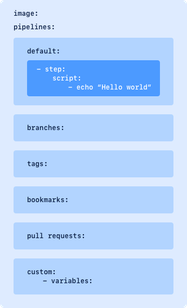
\includegraphics[width=0.3\linewidth]{Foto's/yml-structure.png}
    \caption{Structureel overzicht van Bitbucket Pipelines. Bron:~\autocite{atlassianConfigure}.}
    \label{fig:Structureel-overzicht}
\end{figure}
\\\\
Bitbucket Pipelines vereist een Bitbucket Cloud-abonnement. De kosten zijn afhankelijk van het aantal gebruikers en de gewenste functies. Build-minuten zijn binnen het abonnement gebundeld tot een bepaald maximum, waarna extra kosten in rekening worden gebracht. Runners stellen gebruikers in staat om pipelines op hun eigen infrastructuur uit te voeren,waarbij de gebruikte minuten niet meetellen voor de kosten. Deze flexibele opzet maakt Bitbucket Pipelines een krachtige tool voor teams die hun ontwikkelingsprocessen willen automatiseren en optimaliseren.~\autocite{atlassianBambooSpecs}~\autocite{atlassianPricing}.

\newpage
\subsubsection{GitLab CI/CD}

GitLab CI/CD is een tool binnen GitLab,  die gebruikers in staat stelt om geautomatiseerde build- en testprocessen uit te voeren op hun code. Om gebruik te maken van deze functionaliteit, is een GitLab-repository vereist. GitLab kan zelfgehost worden en beheerd op  eigen servers, of gekocht worden als een abonnementsgebaseerde SaaS-oplossing. Om GitLab CI/CD te gebruiken, moet er een runner beschikbaar zijn. Runners kunnen door GitLab worden gehost of zelfgehost worden. Deze runner is verantwoordelijk voor het uitvoeren van de taken die in een pipeline zijn gedefinieerd~\autocite{gitlabRunner}~\autocite{gitlabCi}. 
\\\\
De configuratie van GitLab CI/CD gebeurt via een YAML-bestand genaamd “gitlab-ci.yml”. In dit bestand definieert de gebruiker verschillende jobs die moeten worden uitgevoerd met behulp van een vooraf gedefinieerde structuur, zoals gedeclareerd in Code 1. Dit gestructureerde formaat maakt het eenvoudig om pipelines op te zetten en aan te passen. In dit voorbeeld wordt de naam van de opdracht opgegeven, waarna de stage van de opdracht wordt gedefinieerd. De sectie ``script" definieert de commando's die in deze stap moeten worden uitgevoerd. De pipeline kan ook gevisualiseerd worden (Figuur 2.6) om een completer begrip van de huidige staat te bieden~\autocite{gitlabPipelines}~\autocite{gitlabRunner}.
\\\\
Code 1 Basis YAML-structuur van GitLab CI/CD
\begin{verbatim}
    test-opdracht:
    stage: test
    script:
    - echo "Deze opdracht zal iets gaan testen"
\end{verbatim}
\\\\
\begin{figure}[H]
    \centering
    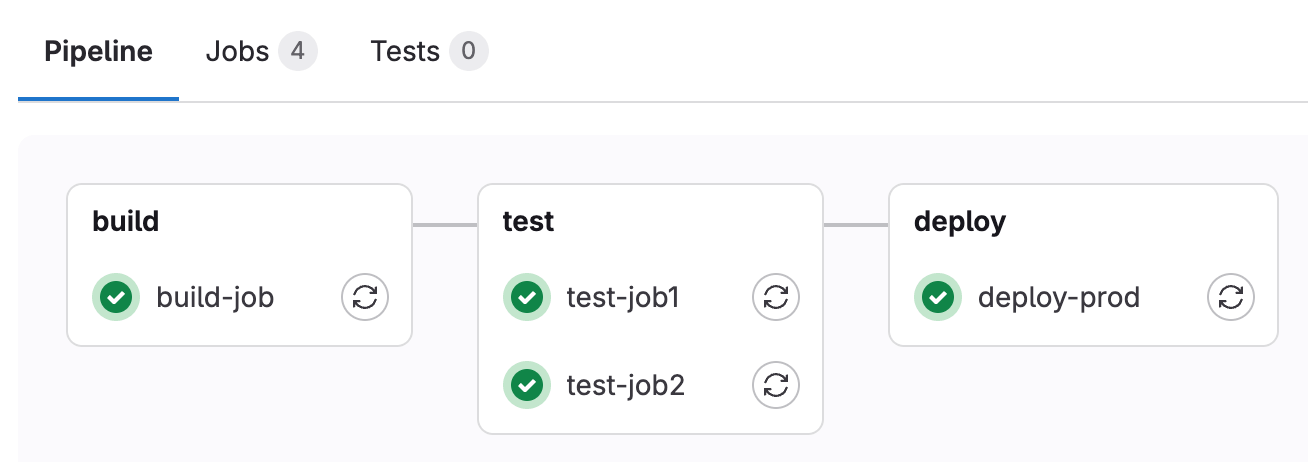
\includegraphics[width=0.8\linewidth]{Foto's/pipeline_graph_v17_9.png}
    \caption{GitLab CI/CD pipeline-status gevisualiseerd. Bron:~\autocite{gitlabPipelines}.}
    \label{fig:pipeline-status}
\end{figure}

\subsubsection{Google Cloud Build}

Google Cloud biedt een serverless CI/CD-dienst genaamd Cloud Build, waarmee gebruikers hun builds kunnen uitvoeren op de infrastructuur van Google Cloud Platform (GCP). Deze service maakt het mogelijk om broncode te importeren vanuit externe repositories of cloudopslag en builds uit te voeren volgens vooraf gedefinieerde specificaties. Cloud Build genereert artefacten en slaat deze op in de configuratie~\autocite{googleCloudBuildOverview}.
\\\\
Builds wordt gedaan met behulp van Google Build Config, die gedetailleerde instructies geeft voor de verschillende fasen en taken die binnen een build moeten worden uitgevoerd. Builds kunnen worden gebruikt om standaard taken in een CI/CD-pipeline uit te voeren, zoals het ophalen van afhankelijkheden, het produceren van builds en het uitvoeren van unittests. Build-configuraties worden geschreven in YAML- of JSON-syntaxis. Een bijzonder kenmerk van Cloud Build is de mogelijkheid om Docker-images te maken op basis van een Dockerfile~\autocite{googleQuickstartBuild}. Cloud Build-pipelines kunnen lokaal getest worden om de Build Config die voor de pipeline is geschreven te testen, met behulp van de tool cloud-build-local, wat helpt om eventuele fouten vroegtijdig te identificeren voordat ze naar de cloud worden gepusht.~\autocite{googleCloudBuildOverview}.
\\\\
De kosten van CI/CD-implementatie op Google Cloud zijn gebaseerd op het aantal build-minuten op de Cloud. Daarnaast kunnen kosten ontstaan door opgeslagen artefacten en het gebruikte netwerkverkeer. Ook Secret Manager draagt bij aan de kosten~\autocite{googleCloudBuildPricing}~\autocite{googleSecretManagerPricing}.

\subsection{Betrouwbaarheid en Onderhoud van de Pipeline}
Een stabiele pipeline vereist continue monitoring en onderhoud om fouten te minimaliseren. Dit kan worden bereikt door:

\begin{itemize}
    \item \textbf{Logging en Monitoring}: fouten detecteren en prestaties te analyseren.
    \item \textbf{Retry Mechanismen}: Automatische herhaalpogingen bij tijdelijke fouten zoals netwerkproblemen.
    \item \textbf{Beveiliging}: API-sleutels en tokens veilig opslaan en versleutelen om ongeautoriseerde toegang te voorkomen.
\end{itemize}

Door deze strategieën toe te passen, kan een efficiënte pipeline worden ontwikkeld die het volledige proces van orderverwerking tot 3D-printing automatiseert.





% Tip: Begin elk hoofdstuk met een paragraaf inleiding die beschrijft hoe
% dit hoofdstuk past binnen het geheel van de bachelorproef. Geef in het
% bijzonder aan wat de link is met het vorige en volgende hoofdstuk.

% Pas na deze inleidende paragraaf komt de eerste sectiehoofding.

%Dit hoofdstuk bevat je literatuurstudie. De inhoud gaat verder op de inleiding, maar zal het onderwerp van de bachelorproef *diepgaand* uitspitten. De bedoeling is dat de lezer na lezing van dit hoofdstuk helemaal op de hoogte is van de huidige stand van zaken (state-of-the-art) in het onderzoeksdomein. Iemand die niet vertrouwd is met het onderwerp, weet nu voldoende om de rest van het verhaal te kunnen volgen, zonder dat die er nog andere informatie moet over opzoeken \autocite{Pollefliet2011}.

%Je verwijst bij elke bewering die je doet, vakterm die je introduceert, enz.\ naar je bronnen. In \LaTeX{} kan dat met het commando \texttt{$\backslash${textcite\{\}}} of \texttt{$\backslash${autocite\{\}}}. Als argument van het commando geef je de ``sleutel'' van een ``record'' in een bibliografische databank in het Bib\LaTeX{}-formaat (een tekstbestand). Als je expliciet naar de auteur verwijst in de zin (narratieve referentie), gebruik je \texttt{$\backslash${}textcite\{\}}. Soms is de auteursnaam niet expliciet een onderdeel van de zin, dan gebruik je \texttt{$\backslash${}autocite\{\}} (referentie tussen haakjes). Dit gebruik je bv.~bij een citaat, of om in het bijschrift van een overgenomen afbeelding, broncode, tabel, enz. te verwijzen naar de bron. In de volgende paragraaf een voorbeeld van elk.

%\textcite{Knuth1998} schreef een van de standaardwerken over sorteer- en zoekalgoritmen. Experten zijn het erover eens dat cloud computing een interessante opportuniteit vormen, zowel voor gebruikers als voor dienstverleners op vlak van informatietechnologie~\autocite{Creeger2009}.

%Let er ook op: het \texttt{cite}-commando voor de punt, dus binnen de zin. Je verwijst meteen naar een bron in de eerste zin die erop gebaseerd is, dus niet pas op het einde van een paragraaf.

%\begin{figure}
  %\centering
  %
\includegraphics[width=0.8\textwidth]{grail.jpg}
  %\caption[Voorbeeld figuur.]{\label{fig:grail}Voorbeeld van invoegen van een figuur. Zorg altijd voor een uitgebreid bijschrift dat de figuur volledig beschrijft zonder in de tekst te moeten gaan zoeken. Vergeet ook je bronvermelding niet!}
%\end{figure}

%\begin{listing}
  %\begin{minted}{python}
    %import pandas as pd
   %% import seaborn as sns

    %penguins = sns.load_dataset('penguins')
   % sns.relplot(data=penguins, x="flipper_length_mm", %y="bill_length_mm", hue="species")
 % \end{minted}
  %\caption[Voorbeeld codefragment]{Voorbeeld van het invoegen van een %codefragment.}
%\end{listing}

%\lipsum[7-20]

%\begin{table}
 % \centering
 % \begin{tabular}{lcr}
   % \toprule
   % \textbf{Kolom 1} & \textbf{Kolom 2} & \textbf{Kolom 3} \\
   % $\alpha$         & $\beta$          & $\gamma$         \\
   % \midrule
   % A                & 10.230           & a                \\
   % B                & 45.678           & b                \\
    %C                & 99.987           & c                \\
   % \bottomrule
 % \end{tabular}
 % \caption[Voorbeeld tabel]{\label{tab:example}Voorbeeld van een tabel.}
%\end{table}

